\section{Definitional disjunction}\label{sec:defdisj}

\Figref{fig:meaningspace} gives the space of meanings that we work in.

Even prior over states.

Include a nonce message that is true in all states.

Assume that the unknown word has an atomic meaning. In this context,
this just means that we asume that the unknown word will either exist
at the same conceptual level as the known words or be identical to one
of them.



\begin{figure}[htp]
  \centering
  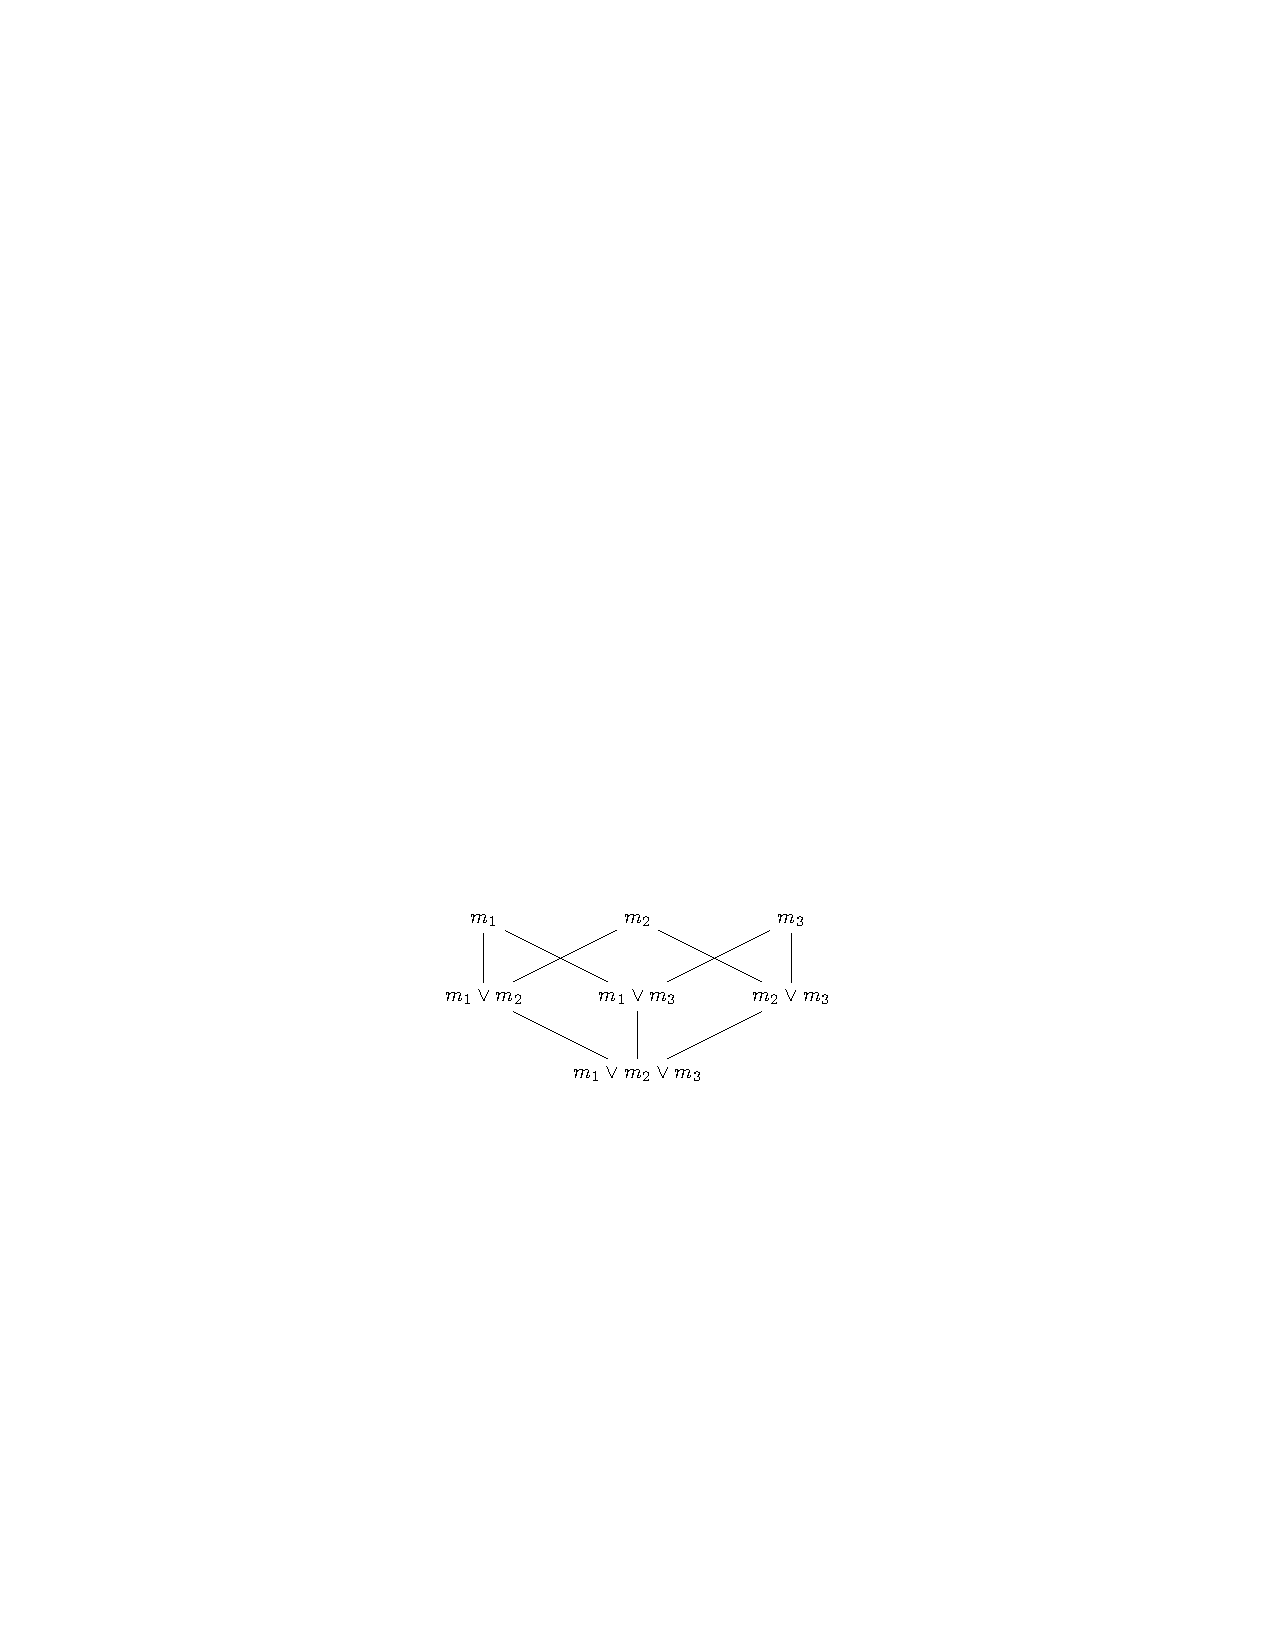
\includegraphics[scale=1]{images/meaningspace}
  \caption{Meaning space.}
  \label{fig:meaningspace}
\end{figure}

\Figref{fig:S3andS4} studies some of the hyperparameters. The
important thing is to connect this with the discourse participants'
mutual, public knowledge about expertise and goals.w


\begin{figure}[htp]
  \centering
  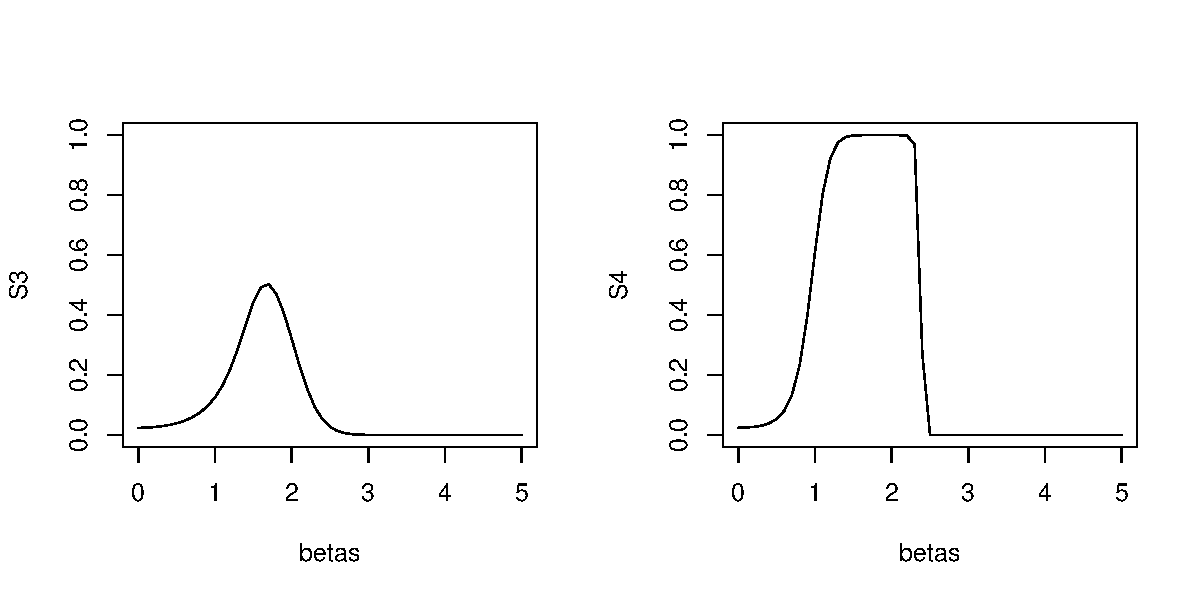
\includegraphics[width=1\textwidth]{images/S3andS4}
  \caption{Hyperparameter exploration.}
  \label{fig:S3andS4}
\end{figure}


%%% Local Variables: 
%%% mode: latex
%%% TeX-master: "definitional_disjunction"
%%% End:
